% !TEX root = main.tex
\section*{Modélisation}

Cette partie décrit la résolution du modèle homogénéisé unidimensionnel. On
présente d'abord deux solutions analytiques obtenues dans des cas réduits,
qui servent de solutions de référence : la solution de Thiele, où seul le
transport de matière limite la réaction, et la solution de Newman et Tobias,
où seule la conduction la limite. On détaille ensuite la discrétisation du
modèle 1D général, puis la résolution du système non linéaire obtenu.

% ============================================================
\subsection*{Solutions analytiques de référence}

\subsubsection*{Cas diffusion--réaction : solution de Thiele}

Dans le cas réduit étudié précédemment (régime stationnaire, transport
purement diffusif, potentiels uniformes et cinétique du premier ordre), le
système admet une solution analytique. Pour le \ce{CO2} et le \ce{CO}, avec
$\zeta = (z - L_m)/l_e \in [0, 1]$, le collecteur en $\zeta = 0$ et
l'interface avec la phase homogène en $\zeta = 1$ :
\begin{align}
\avg{C_{\ce{CO2}}}^l(\zeta)
&= C_{\ce{CO2}}^{\mathrm{hom}}\,
\frac{\cosh(\phi\zeta)}{\cosh(\phi)},
\label{eq:ref_CO2}\\
\avg{C_{\ce{CO}}}^l(\zeta)
&= C_{\ce{CO}}^{\mathrm{hom}}
+ \frac{D_{\ce{CO2}}^{\mathrm{eff}}}{D_{\ce{CO}}^{\mathrm{eff}}}\,
C_{\ce{CO2}}^{\mathrm{hom}}
\left[1 - \frac{\cosh(\phi\zeta)}{\cosh(\phi)}\right],
\label{eq:ref_CO}
\end{align}
et le facteur d'efficacité vaut $\eta_E = \tanh(\phi)/\phi$.

Cette solution joue deux rôles dans la suite.
\begin{itemize}
    \item \textbf{Vérification du code.} Le modèle numérique général doit
    redonner exactement \eqref{eq:ref_CO2}--\eqref{eq:ref_CO} lorsqu'on y
    impose les mêmes hypothèses : espèces neutres, conductivités très grandes
    et cinétique linéarisée. L'écart entre solution numérique et solution
    analytique permet de mesurer l'erreur de discrétisation et de vérifier
    l'ordre de convergence du schéma lorsque le maillage est raffiné.
    \item \textbf{Choix du maillage.} Pour $\phi \gg 1$, la réaction est
    confinée dans une couche d'épaisseur $l_e/\phi$ près de l'interface avec
    la phase homogène, où la concentration varie fortement. Le maillage doit
    résoudre cette couche, ce qui justifie un raffinement près de $z = L_b$.
\end{itemize}

\subsubsection*{Cas conduction : solution de Newman et Tobias}

La solution de Thiele suppose les potentiels uniformes : elle ne dit rien de
la conduction dans le solide et dans l'électrolyte. Le cas réduit inverse,
où les concentrations sont uniformes et où seules les résistances des deux
phases limitent la réaction, admet lui aussi une solution analytique,
établie par Newman et Tobias~\cite{newman1962}. On la déduit ici du modèle
1D~\eqref{eq:flux1D}--\eqref{eq:charge1D} en deux hypothèses.

\paragraph{Hypothèse 1 : concentrations uniformes.} Si la diffusion est très
rapide devant la réaction, les concentrations restent égales à leur valeur
dans la phase homogène, $C_i = C_i^{\mathrm{hom}}$. Le flux~\eqref{eq:flux1D}
se réduit alors à la migration, et le courant ionique
$i_l = F\sum_i z_i N_i$ suit une loi d'Ohm :
\begin{equation}
i_l = -\kappa\,\frac{\partial \varphi_l}{\partial z},
\qquad
\kappa = \frac{F^2}{RT}\sum_i z_i^2\,\varepsilon_l D_i^{\mathrm{eff}}\,C_i^{\mathrm{hom}} .
\label{eq:NT_kappa}
\end{equation}
De même, on note $i_s = -K_s\,\partial\varphi_s/\partial z$ le courant
électronique, avec $K_s = \varepsilon_s\sigma^{\mathrm{eff}}$. On suppose en
outre $C_{\ce{CO2}}^{\mathrm{hom}} = C_{\ce{CO}}^{\mathrm{hom}} = C_{\mathrm{ref}}$,
de sorte que la surtension
$\eta = \varphi_s - \varphi_l - E_{\mathrm{eq}}^{\mathrm{ref}}$ soit nulle à
l'équilibre. Cette hypothèse correspond à la limite opposée du cas de Thiele :
le module de Thiele est très petit, $\phi \ll 1$, et le facteur d'efficacité
de Thiele vaut $\eta_E = \tanh(\phi)/\phi \simeq 1$. Le transport de matière
n'entraîne alors aucune perte, et seule la conduction peut limiter la
réaction.

\paragraph{Conservation du courant total.} D'après~\eqref{eq:ohm1D}
et~\eqref{eq:charge1D}, $\partial i_s/\partial z = a\,j$ et
$\partial i_l/\partial z = -a\,j$ : ce que la réaction retire au solide, elle
le donne à l'électrolyte, et $i_s + i_l = I$ est constant. Au collecteur, le
flux de chaque espèce est nul, donc $i_l = 0$ et tout le courant circule dans
le solide, $i_s = I$ ; à l'interface avec la phase homogène,
$\partial\varphi_s/\partial z = 0$, donc $i_s = 0$ et $i_l = I$.

\paragraph{Hypothèse 2 : cinétique linéaire.} Pour une faible surtension,
$|F\eta/RT| \ll 1$, le développement au premier ordre de la loi de
Butler--Volmer donne
\begin{equation}
a\,j \simeq -k\,\eta,
\qquad
k = a\,j_{0,\mathrm{ref}}\,(\alpha_a + \alpha_c)\,\frac{F}{RT} .
\end{equation}

\paragraph{Équation sur la surtension.} En dérivant
$\eta = \varphi_s - \varphi_l - E_{\mathrm{eq}}^{\mathrm{ref}}$, il vient
\begin{equation}
\frac{\partial\eta}{\partial z} = -\frac{i_s}{K_s} + \frac{i_l}{\kappa},
\qquad
\frac{\partial^2\eta}{\partial z^2}
= -a\,j\left(\frac{1}{K_s} + \frac{1}{\kappa}\right)
= k\left(\frac{1}{K_s} + \frac{1}{\kappa}\right)\eta .
\label{eq:NT_derivee}
\end{equation}
Avec $\zeta = (z - L_m)/l_e$, on obtient
\begin{equation}
\frac{\mathrm{d}^2\eta}{\mathrm{d}\zeta^2} = \Lambda^2\,\eta,
\qquad
\Lambda^2 = k\,l_e^2\left(\frac{1}{\kappa} + \frac{1}{K_s}\right),
\end{equation}
où le nombre adimensionnel $\Lambda$ joue pour la conduction le rôle que joue
le module de Thiele $\phi$ pour le transport de matière. D'après le bilan de
courant aux deux bords, les conditions limites portent sur la dérivée :
\begin{equation}
\left.\frac{\mathrm{d}\eta}{\mathrm{d}\zeta}\right|_{\zeta=0} = -\frac{I\,l_e}{K_s},
\qquad
\left.\frac{\mathrm{d}\eta}{\mathrm{d}\zeta}\right|_{\zeta=1} = \frac{I\,l_e}{\kappa} .
\end{equation}

\paragraph{Solution.} En écrivant $\eta = A\cosh(\Lambda\zeta) + B\sinh(\Lambda\zeta)$
et en appliquant ces deux conditions, on obtient
\begin{equation}
\eta(\zeta) = \frac{I\,l_e}{\Lambda}
\left[
\left(\frac{1}{\kappa} + \frac{\cosh\Lambda}{K_s}\right)
\frac{\cosh(\Lambda\zeta)}{\sinh\Lambda}
- \frac{\sinh(\Lambda\zeta)}{K_s}
\right].
\label{eq:ref_NT}
\end{equation}
La réaction se concentre près des deux bords : du côté du collecteur, où le
courant électronique est le plus fort, et du côté de la phase homogène, où le
courant ionique est le plus fort.

\paragraph{Relation avec le potentiel imposé.} Le calcul n'impose pas le
courant $I$, mais les potentiels $\varphi_s = E$ au collecteur et
$\varphi_l = \varphi_l^{\mathrm{hom}}$ à l'interface. La tension imposée
$V = E - \varphi_l^{\mathrm{hom}} - E_{\mathrm{eq}}^{\mathrm{ref}}$ n'est pas
la surtension locale : elle comprend en plus la chute de potentiel dans
l'électrolyte,
\begin{equation}
V = \eta(0) + \left[\varphi_l(0) - \varphi_l(1)\right] .
\end{equation}
En combinant~\eqref{eq:NT_derivee} et $i_s = I - i_l$, on obtient
$i_l = (\partial\eta/\partial z + I/K_s)\,K_s\kappa/(K_s + \kappa)$, dont
l'intégration sur l'électrode donne la chute de potentiel :
\begin{equation}
\varphi_l(0) - \varphi_l(1)
= \frac{K_s}{K_s + \kappa}\left[\eta(1) - \eta(0) + \frac{I\,l_e}{K_s}\right] .
\end{equation}
En y reportant $\eta(0)$ et $\eta(1)$ tirés de~\eqref{eq:ref_NT}, on trouve
$V = R_{\mathrm{el}}\,I$, avec la résistance de l'électrode
\begin{equation}
R_{\mathrm{el}} = \frac{l_e}{K_s + \kappa}
\left[1 + \frac{2 + \left(\kappa/K_s + K_s/\kappa\right)\cosh\Lambda}{\Lambda\sinh\Lambda}\right] .
\label{eq:NT_R}
\end{equation}
Le courant $I = V/R_{\mathrm{el}}$ et le profil~\eqref{eq:ref_NT} sont ainsi
entièrement déterminés par les données : la solution de référence ne dépend
d'aucun résultat du calcul.

\paragraph{Facteur d'efficacité.} Par analogie avec Thiele, on compare le
courant au courant obtenu si toute l'électrode voyait la surtension $V$,
$-k\,V\,l_e$ :
\begin{equation}
\eta_E^{\mathrm{NT}} = \frac{I}{-k\,V\,l_e} = \frac{1}{k\,l_e\,R_{\mathrm{el}}} .
\end{equation}
La perte d'efficacité ne vient plus ici de l'appauvrissement en réactif,
puisque $\eta_E = 1$, mais des chutes de potentiel dans les deux phases.

\paragraph{Généralisation.} Si $C_{\ce{CO2}}^{\mathrm{hom}} \neq C_{\ce{CO}}^{\mathrm{hom}}$,
toutes deux non nulles, l'équilibre est décalé de
\begin{equation*}
\eta_{\mathrm{eq}} = \frac{RT}{(\alpha_a + \alpha_c)F}\,
\ln\!\left(\frac{C_{\ce{CO2}}^{\mathrm{hom}}}{C_{\ce{CO}}^{\mathrm{hom}}}\right),
\end{equation*}
et la même démarche s'applique à $\eta - \eta_{\mathrm{eq}}$, avec une
constante $k$ modifiée. En revanche, si $C_{\ce{CO}}^{\mathrm{hom}} = 0$, il
n'existe pas d'équilibre et la linéarisation n'est pas possible.

% ============================================================
\subsection*{Discrétisation du modèle 1D}

\subsubsection*{Système à discrétiser}

On discrétise le système unidimensionnel~\eqref{eq:proj_flux}--\eqref{eq:proj_ohm}
obtenu par projection sur la direction normale à l'électrode, sur
$z \in [L_m, L_b]$. Pour la configuration étudiée, à collecteur plein, la
vitesse superficielle normale est nulle, $u = 0$ : le flux ne contient que
la diffusion et la migration. Le coefficient $D_i^{\mathrm{tot}}$ peut
inclure une dispersion transverse due à un écoulement latéral. Une électrode
traversée par l'électrolyte demanderait d'ajouter un terme convectif $u\,C_i$
au flux, ainsi qu'une condition d'entrée du fluide au collecteur. On retient la fermeture $\vec{d} = \vec{b}$, qui donne
$D_i^{\mathrm{eff,mig}} = D_i^{\mathrm{eff}}$. Pour alléger l'écriture, on
note $C_i$ la concentration moyenne intrinsèque $\avg{C_i}^l$, $\varphi_l$ et
$\varphi_s$ les potentiels moyens, $j$ la densité de courant
$\avg{j}^{sf}$ et $a = a_v^{\mathrm{cat}}$. On introduit le potentiel
électrolytique adimensionné $\varphi_l^* = F\varphi_l/(RT)$.

Le flux de l'espèce $i$ s'écrit alors :
\begin{equation}
N_i = - D_i^{\mathrm{tot}}\,\frac{\partial C_i}{\partial z}
- \varepsilon_l D_i^{\mathrm{eff}}\, z_i C_i\,\frac{\partial \varphi_l^*}{\partial z},
\label{eq:flux1D}
\end{equation}
et le système à résoudre est :
\begin{align}
\varepsilon_l\frac{\partial C_i}{\partial t} + \frac{\partial N_i}{\partial z}
&= a\,\frac{\nu_i}{n_eF}\,j,
\label{eq:bilan1D}\\
\sum_i z_i C_i &= 0,
\label{eq:EN1D}\\
\frac{\partial}{\partial z}\left(\varepsilon_s\sigma^{\mathrm{eff}}\,
\frac{\partial \varphi_s}{\partial z}\right) &= -a\,j,
\label{eq:ohm1D}
\end{align}
avec $j = j\left(C_{\ce{CO2}},\, C_{\ce{CO}},\,
\varphi_s - \varphi_l - E_{\mathrm{eq}}^{\mathrm{ref}}\right)$ donné par la
loi de Butler--Volmer.

Les conditions limites sont :
\begin{itemize}
    \item au collecteur, $z = L_m$ : $N_i = 0$, sur le flux total (diffusion
    et migration), et $\varphi_s = E$ ;
    \item à l'interface avec la phase homogène, $z = L_b$ :
    $C_i = C_i^{\mathrm{hom}}$, $\varphi_l = \varphi_l^{\mathrm{hom}}$ et
    $\partial\varphi_s/\partial z = 0$.
\end{itemize}

Comme dans le modèle local, l'électroneutralité ne contient pas
$\varphi_l$. L'équation qui détermine le potentiel électrolytique est la
conservation du courant ionique, obtenue en sommant les bilans pondérés par
$z_iF$ :
\begin{equation}
\frac{\partial i_l}{\partial z} = -a\,j,
\qquad i_l = F\sum_i z_i N_i ,
\label{eq:charge1D}
\end{equation}
Le terme d'accumulation a disparu par électroneutralité : cette équation ne
contient pas de dérivée temporelle. Comme elle est une combinaison des bilans,
on ne peut pas conserver à la fois tous les bilans et cette équation : le
bilan d'une espèce chargée $q$, choisie parmi les ions qui ne réagissent pas,
est remplacé par l'électroneutralité~\eqref{eq:EN1D}. Toutes les
concentrations sont conservées comme inconnues. On a ainsi en chaque point
$N+2$ inconnues, les $N$ concentrations, $\varphi_l$ et $\varphi_s$, et
$N+2$ équations : $N-1$ bilans d'espèces, l'électroneutralité, la
conservation du courant ionique et la loi d'Ohm.

\subsubsection*{Maillage et volumes finis}

On utilise une méthode des volumes finis, qui écrit les bilans sur des
volumes de contrôle et conserve donc exactement la matière et la charge au
niveau discret. On reprend les notations du modèle du semi-conducteur. Le domaine
$[L_m, L_b]$ est discrétisé en $M$ nœuds de positions
\begin{equation}
L_m = z_0 < z_1 < \dots < z_{M-1} = L_b ,
\end{equation}
la lettre $N$ étant ici réservée au nombre d'espèces. Le maillage est soit
uniforme, soit raffiné aux deux bords du domaine, là où les gradients sont
les plus forts : près de $z = L_b$, où se concentre la réaction lorsque le
module de Thiele est grand, et près du collecteur. Dans le second cas, chaque
moitié du domaine est découpée en mailles de taille croissante en progression
géométrique de raison $r > 1$, depuis une première maille inférieure ou égale
à $h_{\min}$ au bord jusqu'au centre ; la seconde moitié est le miroir de la
première. La valeur $r = 1$ redonne un maillage uniforme de pas inférieur ou
égal à $h_{\min}$. On note
$h_k = z_{k+1} - z_k$ le pas entre deux nœuds consécutifs. La méthode des
volumes finis associe à chaque nœud un volume de contrôle $\omega_k$, défini
comme la demi-distance aux voisins :
\begin{equation}
\omega_k = \frac{z_{k+1} - z_{k-1}}{2}
\quad\text{(nœud intérieur)},
\qquad
\omega_0 = \frac{h_0}{2},
\qquad
\omega_{M-1} = \frac{h_{M-2}}{2},
\label{eq:omega_ec}
\end{equation}
les volumes des deux nœuds de bord étant des demi-volumes. Le volume de
contrôle du nœud $k$ s'étend de $z_k - h_{k-1}/2$ à $z_k + h_k/2$ : ses faces
sont situées au milieu des intervalles. On note $N_{i,k+1/2}$ le flux de
l'espèce $i$ à travers la face située au milieu de l'intervalle
$[z_k, z_{k+1}]$, c'est-à-dire la face droite du volume de contrôle du
nœud $k$ ; $N_{i,k-1/2}$ est le flux à travers sa face gauche.

\subsubsection*{Bilans discrets}

On intègre chaque équation sur le volume de contrôle du nœud $k$. Pour
l'espèce $i$, la variation de la quantité contenue dans le volume est égale
au flux entrant par la face gauche, moins le flux sortant par la face droite,
plus la production par la réaction :
\begin{equation}
\varepsilon_l\, \omega_k\, \frac{C_{i,k}^{n+1} - C_{i,k}^{n}}{\Delta t}
+ N_{i,k+1/2} - N_{i,k-1/2}
= a\, \omega_k\, \frac{\nu_i}{n_eF}\, j_k ,
\label{eq:bilan_discret}
\end{equation}
où l'exposant $n$ désigne le pas de temps. Tous les termes de droite et les
flux sont évalués au pas $n+1$ (schéma d'Euler implicite), ce qui rend le
schéma stable quel que soit $\Delta t$. Pour un calcul stationnaire, le terme
temporel est simplement supprimé ; c'est le cas traité par le code présenté
dans la suite.

Le terme source est intégré sur le volume de contrôle en supposant la densité
de courant uniforme sur celui-ci et égale à sa valeur au nœud, d'où le
produit $\omega_k\, j_k$. Cette valeur est donnée par la loi de
Butler--Volmer~\eqref{eq:BV}, évaluée avec les inconnues du nœud $k$ :
\begin{equation}
j_k = j_{0,\mathrm{ref}}
\left[
\frac{C_{\ce{CO2},k}}{C_{\ce{CO2}}^{\mathrm{ref}}}
\exp\!\left(-\frac{\alpha_c F \eta_k}{RT}\right)
-
\frac{C_{\ce{CO},k}}{C_{\ce{CO}}^{\mathrm{ref}}}
\exp\!\left(\frac{\alpha_a F \eta_k}{RT}\right)
\right],
\qquad
\eta_k = \varphi_{s,k} - \varphi_{l,k} - E_{\mathrm{eq}}^{\mathrm{ref}} .
\label{eq:BV_discret}
\end{equation}
La densité de courant au nœud $k$ ne dépend que des inconnues de ce même
nœud : $C_{\ce{CO2},k}$, $C_{\ce{CO},k}$, $\varphi_{s,k}$ et $\varphi_{l,k}$.
Dans la jacobienne, elle ne contribue donc qu'aux blocs diagonaux. Dans
l'implémentation actuelle, une même concentration de référence $C_{\mathrm{ref}}$
est utilisée pour le \ce{CO2} et pour le \ce{CO}.

La conservation du courant ionique s'écrit de même, sans terme temporel :
\begin{equation}
F\sum_i z_i\left(N_{i,k+1/2} - N_{i,k-1/2}\right) = -a\, \omega_k\, j_k ,
\label{eq:charge_discret}
\end{equation}
ce qui est exactement la combinaison des bilans
discrets~\eqref{eq:bilan_discret} pondérés par $z_iF$. Le système discret
conserve donc la même structure que le système continu.

La loi d'Ohm est discrétisée par des différences centrées, le courant
électronique à travers une face étant proportionnel à la différence de
potentiel entre les deux nœuds voisins :
\begin{equation}
\varepsilon_s\sigma^{\mathrm{eff}}
\left(
\frac{\varphi_{s,k+1} - \varphi_{s,k}}{h_k}
-
\frac{\varphi_{s,k} - \varphi_{s,k-1}}{h_{k-1}}
\right)
= -a\, \omega_k\, j_k .
\label{eq:ohm_discret}
\end{equation}

\subsubsection*{Flux aux faces : différences centrées}

Il reste à exprimer le flux $N_{i,k+1/2}$ à la face entre les nœuds $k$ et
$k+1$. On utilise des différences centrées : les dérivées sont remplacées par
la différence des valeurs aux deux nœuds divisée par leur distance, et les
concentrations qui multiplient le champ sont prises égales à la moyenne des
deux nœuds :
\begin{equation}
N_{i,k+1/2} =
- D_i^{\mathrm{tot}}\,\frac{C_{i,k+1} - C_{i,k}}{h_k}
- \varepsilon_l D_i^{\mathrm{eff}}\, z_i\, \bar{C}_{i,k+1/2}\,
\frac{\varphi_{l,k+1}^* - \varphi_{l,k}^*}{h_k},
\label{eq:flux_centre}
\end{equation}
où $\bar{C}_{i,k+1/2} = (C_{i,k} + C_{i,k+1})/2$. Ce schéma est précis au
second ordre sur un maillage uniforme et simple à dériver, ce qui facilite la
construction de la jacobienne. Pour les espèces neutres, il
se réduit à la diffusion pure et traite le \ce{CO2} et le \ce{CO} exactement
comme dans le cas analytique.

\paragraph{Condition de validité.} Le schéma centré n'est fiable que si la
diffusion reste prépondérante à l'échelle d'une maille. On mesure
l'importance relative de la migration par le nombre de Péclet de maille :
\begin{equation}
\mathrm{Pe}_{i,k+1/2} = z_i\,\frac{\varepsilon_l D_i^{\mathrm{eff}}}{D_i^{\mathrm{tot}}}
\left(\varphi_{l,k+1}^* - \varphi_{l,k}^*\right) .
\label{eq:peclet_maille}
\end{equation}
Il faut $|\mathrm{Pe}_{i,k+1/2}| < 2$ sur chaque maille et pour chaque espèce.
Au-delà, la migration l'emporte sur la diffusion à l'échelle de
la maille : dans l'équation discrète, le coefficient qui relie un nœud à son
voisin change de signe, et la solution peut présenter des oscillations non
physiques, voire des concentrations négatives. En pratique, on calcule
$\max|\mathrm{Pe}_{i,k+1/2}|$ après chaque résolution. Si la condition n'est pas
respectée, on raffine le maillage là où elle est violée, ou l'on passe au
schéma de Scharfetter--Gummel décrit ci-dessous.

Pour fixer les ordres de grandeur, cette condition impose une chute de
potentiel inférieure à environ $2RT/F \approx 50$~mV entre deux nœuds, ce qui
est en général largement vérifié dans l'électrolyte.

\subsubsection*{Option : schéma de Scharfetter--Gummel}

Lorsque la migration devient importante, il est plus
efficace de changer de schéma que de raffiner fortement le maillage. Le
schéma de Scharfetter--Gummel, déjà employé pour le solveur de
dérive--diffusion des semi-conducteurs, s'applique directement : le flux de
Nernst--Planck a la même structure, la migration jouant le rôle de la dérive.

Pour le voir, on réécrit le flux~\eqref{eq:flux1D} sous la forme
\begin{equation}
N_i = -D_i^{\mathrm{tot}}\left(\frac{\partial C_i}{\partial z}
+ C_i\,\frac{\partial g_i}{\partial z}\right),
\qquad
\frac{\partial g_i}{\partial z} =
z_i\,\frac{\varepsilon_l D_i^{\mathrm{eff}}}{D_i^{\mathrm{tot}}}\,
\frac{\partial \varphi_l^*}{\partial z} ,
\end{equation}
où $g_i$ traduit l'effet du champ électrique. Le
principe du schéma est de supposer, sur l'intervalle $[z_k, z_{k+1}]$, que le
flux $N_i$ est constant, que les coefficients sont constants et que le
potentiel varie linéairement. L'équation du flux devient alors une équation
différentielle du premier ordre en $C_i$, que l'on intègre exactement. On
obtient :
\begin{equation}
N_{i,k+1/2} =
\frac{D_i^{\mathrm{tot}}}{h_k}
\left[
C_{i,k}\,\mathcal{B}(\mathrm{Pe}_{i,k+1/2}) - C_{i,k+1}\,\mathcal{B}(-\mathrm{Pe}_{i,k+1/2})
\right],
\label{eq:SG}
\end{equation}
où $\mathrm{Pe}_{i,k+1/2}$ est le nombre de Péclet de maille
défini en~\eqref{eq:peclet_maille}, et $\mathcal{B}$ la fonction de Bernoulli :
\begin{equation}
\mathcal{B}(x) = \frac{x}{e^{x} - 1}, \qquad \mathcal{B}(0) = 1 .
\end{equation}

Ce flux possède les bonnes limites physiques :
\begin{itemize}
    \item en l'absence de migration ($\mathrm{Pe}_{i,k+1/2} = 0$), il se réduit
    à la différence centrée
    $D_i^{\mathrm{tot}}\,(C_{i,k} - C_{i,k+1})/h_k$ : on retrouve
    la diffusion pure, et le \ce{CO2} et le \ce{CO} sont traités exactement
    comme dans le cas analytique ;
    \item pour une concentration uniforme, il redonne le flux de migration
    $-\varepsilon_l D_i^{\mathrm{eff}}\, z_i C_i\,
    (\varphi_{l,k+1}^* - \varphi_{l,k}^*)/h_k$ ;
    \item lorsque la migration domine ($|\mathrm{Pe}_{i,k+1/2}| \gg 1$), il
    devient un schéma décentré amont : la concentration utilisée est celle du
    nœud d'où viennent les ions, ce qui garantit des concentrations
    positives. Par exemple, pour un cation entraîné vers les $z$ croissants
    par un fort champ électrique, seule $C_{i,k}$ intervient dans le flux.
\end{itemize}
En pratique, $\mathcal{B}(x)$ est évaluée par un développement limité,
$\mathcal{B}(x) \simeq 1 - x/2 + x^2/12$, lorsque $|x|$ est petit, afin d'éviter la
division $0/0$.

Le schéma centré~\eqref{eq:flux_centre} correspond au développement de
\eqref{eq:SG} au premier ordre en $\mathrm{Pe}_{i,k+1/2}$ : les deux schémas coïncident lorsque
la diffusion domine, et Scharfetter--Gummel reste valable sans condition sur
$|\mathrm{Pe}_{i,k+1/2}|$. Il est en revanche plus coûteux à dériver pour la jacobienne, en raison
de la fonction de Bernoulli.

\subsubsection*{Conditions limites discrètes}

Les conditions limites s'intègrent dans les volumes de contrôle des deux
nœuds de bord, qui sont des demi-volumes : la face externe de chacun d'eux
coïncide avec la frontière du domaine. Aucun nœud fictif n'est donc
nécessaire.

\paragraph{Collecteur, nœud $0$ ($z = L_m$).} Le flux à travers la face
externe est le flux à travers le collecteur, imposé nul :
$N_{i,-1/2} = 0$. Le bilan de chaque espèce $i \neq q$ sur le demi-volume
$\omega_0 = h_0/2$ et la conservation du courant s'écrivent :
\begin{align}
\varepsilon_l\,\omega_0\,\frac{C_{i,0}^{n+1} - C_{i,0}^{n}}{\Delta t}
+ N_{i,1/2} &= a\,\omega_0\,\frac{\nu_i}{n_eF}\,j_0 ,
\label{eq:CL0_espece}\\
F\sum_i z_i\,N_{i,1/2} &= -a\,\omega_0\,j_0 ,
\label{eq:CL0_charge}
\end{align}
où $N_{i,1/2}$ est donné par~\eqref{eq:flux_centre} et ne fait intervenir
que les nœuds $0$ et $1$. Le potentiel solide est imposé, $\varphi_{s,0} = E$,
et le bilan de l'espèce $q$ est remplacé par l'électroneutralité,
$\sum_i z_i C_{i,0} = 0$.

\paragraph{Interface avec la phase homogène, nœud $M-1$ ($z = L_b$).} Les
concentrations et le potentiel électrolytique sont imposés :
\begin{equation}
C_{i,M-1} = C_i^{\mathrm{hom}}, \qquad
\varphi_{l,M-1} = \varphi_l^{\mathrm{hom}},
\label{eq:CLM_dirichlet}
\end{equation}
les concentrations $C_i^{\mathrm{hom}}$ vérifiant l'électroneutralité. Pour
le potentiel solide, le courant électronique à travers la face externe est
nul, et le bilan sur le demi-volume $\omega_{M-1} = h_{M-2}/2$ ne conserve que
le flux de la face gauche :
\begin{equation}
\varepsilon_s\sigma^{\mathrm{eff}}\,
\frac{\varphi_{s,M-1} - \varphi_{s,M-2}}{h_{M-2}}
= a\,\omega_{M-1}\, j_{M-1} ,
\label{eq:CLM_ohm}
\end{equation}
où $j_{M-1}$ est évaluée avec les valeurs imposées $C_i^{\mathrm{hom}}$ et
$\varphi_l^{\mathrm{hom}}$.

\subsubsection*{Système non linéaire}

En rassemblant les inconnues de tous les nœuds dans un vecteur $U$, les
équations~\eqref{eq:bilan_discret}, \eqref{eq:charge_discret},
\eqref{eq:ohm_discret} et les conditions limites forment, à chaque pas de
temps, un système de $(N+2)M$ équations algébriques, noté
\begin{equation}
\mathcal{F}(U) = 0 .
\end{equation}

Ce système est non linéaire, pour deux raisons : le flux de migration fait
intervenir le produit de la concentration et du gradient de potentiel, et la
loi de Butler--Volmer dépend exponentiellement de la surtension. Avec le
schéma de Scharfetter--Gummel, le flux dépend en outre du potentiel de façon
exponentielle. Il est résolu par
la méthode de Newton, qui nécessite la matrice jacobienne
$\partial\mathcal{F}/\partial U$. Comme chaque équation ne fait intervenir
que le nœud $k$ et ses deux voisins, cette matrice est tridiagonale par blocs,
chaque bloc étant de taille $(N+2)\times(N+2)$.

% ============================================================
\subsection*{Déroulement du calcul}

Le calcul stationnaire se déroule en deux temps
(figure~\ref{fig:logigramme_newton}). Une phase de préparation lit les
données, construit le maillage et initialise l'état par la solution de
Thiele. La méthode de Newton est ensuite itérée : à chaque itération, le
résidu et la jacobienne sont assemblés, le système linéaire est résolu, et
l'état est mis à jour avec une correction amortie. Le calcul s'arrête dès que
les corrections deviennent inférieures aux tolérances, ou échoue si le
système linéaire ne peut pas être résolu ou si le nombre maximal d'itérations
est atteint. Les sections suivantes détaillent chacune de ces étapes.

% Logigramme du calcul stationnaire (main.c, newton.c)
% Nécessite dans le préambule : \usetikzlibrary{shapes.geometric}
\begin{figure}[H]
\centering
\begin{tikzpicture}[
    node distance = 0.45cm and 1.0cm,
    >={Stealth[length=2.2mm]},
    etape/.style  = {rectangle, rounded corners=2pt, draw=black!70, fill=blue!6,
                     minimum width=7cm, minimum height=0.75cm, align=center,
                     font=\small},
    debut/.style  = {etape, fill=black!8},
    test/.style   = {diamond, aspect=2.6, draw=black!70, fill=orange!10,
                     inner sep=1pt, align=center, font=\small},
    sortie/.style = {rectangle, rounded corners=2pt, draw=black!70,
                     minimum width=3.2cm, minimum height=0.8cm, align=center,
                     font=\small},
    fleche/.style = {->, thick, draw=black!75},
    etiq/.style   = {font=\footnotesize, fill=white, inner sep=1pt}
]

% ---------------- Préparation ----------------
\node[debut] (lecture) {Lecture des données\\ \texttt{donnees.ini}};
\node[etape, below=of lecture] (maillage) {Construction du maillage\\ nœuds $z_k$, pas $h_k$, volumes $\omega_k$};
\node[etape, below=of maillage] (init) {Initialisation par la solution de Thiele\\ $U^{(0)}$, puis $m = 0$};

% ---------------- Boucle de Newton ----------------
\node[etape, below=0.75cm of init] (assemblage) {Assemblage du résidu $\mathcal{F}(U^{(m)})$\\ et de la jacobienne $J(U^{(m)})$};
\node[etape, below=of assemblage] (echelle) {Mise à l'échelle des lignes de $J$ et de $\mathcal{F}$};
\node[etape, below=of echelle] (resolution) {Résolution de $J\,\delta U = -\mathcal{F}$\\ (Gauss bande, pivot partiel)};
\node[test, below=of resolution] (fini) {Résolution possible\\ et $\delta U$ fini ?};
\node[etape, below=of fini] (maj) {Mise à jour amortie\\ $U^{(m+1)} = U^{(m)} + \delta U$ amorti};
\node[test, below=of maj] (conv) {$\max|\delta C| < \mathrm{tol}_C$\\ et $\max|\delta\varphi| < \mathrm{tol}_\varphi$ ?};
\node[test, below=of conv] (iter) {$m + 1 < m_{\max}$ ?};

% ---------------- Sorties ----------------
\node[sortie, fill=green!10, right=of conv] (succes) {Écriture des profils\\ \texttt{profils.csv}};
\node[sortie, fill=red!10, right=of fini]   (echec)  {Échec\\ pas de convergence};

% ---------------- Flèches principales ----------------
\draw[fleche] (lecture)    -- (maillage);
\draw[fleche] (maillage)   -- (init);
\draw[fleche] (init)       -- (assemblage);
\draw[fleche] (assemblage) -- (echelle);
\draw[fleche] (echelle)    -- (resolution);
\draw[fleche] (resolution) -- (fini);
\draw[fleche] (fini)       -- node[etiq, right] {oui} (maj);
\draw[fleche] (maj)        -- (conv);
\draw[fleche] (conv)       -- node[etiq, right] {non} (iter);

% ---------------- Sorties ----------------
\draw[fleche] (conv) -- node[etiq, above] {oui} (succes);
\draw[fleche] (fini) -- node[etiq, above] {non} (echec);
\coordinate (cote) at ([xshift=0.7cm]succes.east);
\draw[fleche] (iter.east) -- node[etiq, pos=0.5, below] {non} (iter.east -| cote)
              -- (echec.east -| cote) -- (echec.east);

% ---------------- Retour de boucle ----------------
\draw[fleche] (iter.west) -- ++(-1.6,0) node[etiq, pos=0.5, below] {oui}
              |- node[etiq, pos=0.25, left] {$m \leftarrow m+1$} (assemblage.west);

\end{tikzpicture}
\caption{Déroulement du calcul stationnaire. Après la préparation (lecture des
données, maillage, initialisation par la solution de Thiele), la méthode de
Newton répète assemblage, résolution et mise à jour amortie jusqu'à ce que les
corrections sur les concentrations et sur les potentiels passent sous leurs
tolérances respectives.}
\label{fig:logigramme_newton}
\end{figure}


% ============================================================
\subsection*{Construction de la jacobienne}

\paragraph{Ordre des inconnues.} Les inconnues sont rangées nœud par nœud :
au nœud $k$ se suivent les $N$ concentrations $C_{0,k}, \dots, C_{N-1,k}$,
puis $\varphi_{l,k}$ et $\varphi_{s,k}$. Les équations sont rangées de la
même façon : la ligne associée à $C_{i,k}$ porte le bilan de l'espèce $i$
(ou l'électroneutralité si $i = q$), la ligne associée à $\varphi_{l,k}$
porte la conservation du courant ionique, et celle associée à
$\varphi_{s,k}$ porte la loi d'Ohm. Avec $n_v = N+2$ inconnues par nœud, le
système compte $n = n_v M$ inconnues.

Chaque équation ne fait intervenir que les inconnues du nœud $k$ et de ses
deux voisins. Avec ce rangement, la jacobienne est donc une matrice bande :
le coefficient $J_{rc}$ est nul dès que $|r - c| > 2n_v - 1$. La matrice a
ainsi $2n_v - 1$ sous-diagonales et $2n_v - 1$ sur-diagonales, et seule
cette bande est stockée. Pour le cas test présenté plus loin ($N = 4$,
$M = 1001$), cela représente environ $6\,000$ inconnues, mais au plus
$4n_v - 1 = 23$ coefficients non nuls par ligne.

\paragraph{Assemblage par contributions élémentaires.} Le résidu
$\mathcal{F}$ et la jacobienne $J = \partial\mathcal{F}/\partial U$ sont
assemblés par la même fonction. Chaque terme des équations discrètes (un flux
de diffusion à travers une face, un flux de migration, un terme de réaction,
l'électroneutralité, un courant électronique) est programmé une seule fois :
il ajoute sa valeur à la ligne concernée de $\mathcal{F}$ et ses dérivées
aux colonnes correspondantes de $J$. Le résidu et la jacobienne ne peuvent
donc pas devenir incohérents l'un avec l'autre. Les dérivées sont calculées
analytiquement ; on les détaille ci-dessous, contribution par contribution.

\paragraph{Flux de diffusion.} Le flux de diffusion de l'espèce $i$ à travers
la face $k+1/2$ s'écrit
\begin{equation*}
N^{\mathrm{diff}}_{i,k+1/2} = -D_i^{\mathrm{tot}}\,\frac{C_{i,k+1} - C_{i,k}}{h_k} .
\end{equation*}
Ses dérivées non nulles sont :
\begin{align*}
\frac{\partial N^{\mathrm{diff}}_{i,k+1/2}}{\partial C_{i,k}} &= \frac{D_i^{\mathrm{tot}}}{h_k} ,\\[0.2cm]
\frac{\partial N^{\mathrm{diff}}_{i,k+1/2}}{\partial C_{i,k+1}} &= -\frac{D_i^{\mathrm{tot}}}{h_k} .
\end{align*}

\paragraph{Flux de migration.} En notant
\begin{equation*}
\mu_i = \varepsilon_l D_i^{\mathrm{eff}}\, z_i\,\frac{F}{RT} ,
\end{equation*}
le flux de migration à travers la face $k+1/2$ s'écrit
\begin{equation*}
N^{\mathrm{mig}}_{i,k+1/2}
= -\mu_i\,\bar{C}_{i,k+1/2}\,\frac{\varphi_{l,k+1} - \varphi_{l,k}}{h_k},
\qquad
\bar{C}_{i,k+1/2} = \frac{C_{i,k} + C_{i,k+1}}{2} .
\end{equation*}
Il dépend des concentrations des deux nœuds et du potentiel électrolytique
des deux nœuds. Ses dérivées sont :
\begin{align*}
\frac{\partial N^{\mathrm{mig}}_{i,k+1/2}}{\partial C_{i,k}}
= \frac{\partial N^{\mathrm{mig}}_{i,k+1/2}}{\partial C_{i,k+1}}
&= -\frac{\mu_i}{2}\,\frac{\varphi_{l,k+1} - \varphi_{l,k}}{h_k} ,\\[0.2cm]
\frac{\partial N^{\mathrm{mig}}_{i,k+1/2}}{\partial \varphi_{l,k+1}}
&= -\frac{\mu_i\,\bar{C}_{i,k+1/2}}{h_k} ,\\[0.2cm]
\frac{\partial N^{\mathrm{mig}}_{i,k+1/2}}{\partial \varphi_{l,k}}
&= \frac{\mu_i\,\bar{C}_{i,k+1/2}}{h_k} .
\end{align*}

\paragraph{Densité de courant de Butler--Volmer.} On note
\begin{equation*}
e_c = \exp\!\left(-\frac{\alpha_c F\eta_k}{RT}\right),
\qquad
e_a = \exp\!\left(\frac{\alpha_a F\eta_k}{RT}\right),
\end{equation*}
de sorte que
\begin{equation*}
j_k = j_{0,\mathrm{ref}}
\left(\frac{C_{\ce{CO2},k}}{C_{\mathrm{ref}}}\,e_c
- \frac{C_{\ce{CO},k}}{C_{\mathrm{ref}}}\,e_a\right) .
\end{equation*}
Ses dérivées par rapport aux concentrations sont :
\begin{align*}
\frac{\partial j_k}{\partial C_{\ce{CO2},k}} &= \frac{j_{0,\mathrm{ref}}\,e_c}{C_{\mathrm{ref}}} ,\\[0.2cm]
\frac{\partial j_k}{\partial C_{\ce{CO},k}} &= -\frac{j_{0,\mathrm{ref}}\,e_a}{C_{\mathrm{ref}}} .
\end{align*}
Sa dérivée par rapport à la surtension est :
\begin{equation*}
\frac{\partial j_k}{\partial \eta_k}
= -j_{0,\mathrm{ref}}\,\frac{F}{RT}
\left(\alpha_c\,\frac{C_{\ce{CO2},k}}{C_{\mathrm{ref}}}\,e_c
+ \alpha_a\,\frac{C_{\ce{CO},k}}{C_{\mathrm{ref}}}\,e_a\right) .
\end{equation*}
Comme $\eta_k = \varphi_{s,k} - \varphi_{l,k} - E_{\mathrm{eq}}^{\mathrm{ref}}$,
les dérivées par rapport aux potentiels s'en déduisent :
\begin{align*}
\frac{\partial j_k}{\partial \varphi_{s,k}} &= \frac{\partial j_k}{\partial \eta_k} ,\\[0.2cm]
\frac{\partial j_k}{\partial \varphi_{l,k}} &= -\frac{\partial j_k}{\partial \eta_k} .
\end{align*}

\paragraph{Électroneutralité.} La ligne de l'espèce $q$ au nœud $k$ s'écrit
\begin{equation*}
\sum_i z_i\,C_{i,k} = 0 .
\end{equation*}
Sa dérivée par rapport à chaque concentration du nœud est simplement :
\begin{equation*}
\frac{\partial}{\partial C_{i,k}}\left(\sum_{i'} z_{i'}\,C_{i',k}\right) = z_i .
\end{equation*}

\paragraph{Courant électronique.} Le courant électronique à travers la face
$k+1/2$ intervient par le terme
\begin{equation*}
\varepsilon_s\sigma^{\mathrm{eff}}\,\frac{\varphi_{s,k+1} - \varphi_{s,k}}{h_k} .
\end{equation*}
Ses dérivées sont :
\begin{align*}
\frac{\partial}{\partial \varphi_{s,k+1}} &= \frac{\varepsilon_s\sigma^{\mathrm{eff}}}{h_k} ,\\[0.2cm]
\frac{\partial}{\partial \varphi_{s,k}} &= -\frac{\varepsilon_s\sigma^{\mathrm{eff}}}{h_k} .
\end{align*}

\paragraph{Valeurs imposées.} Pour les concentrations et $\varphi_l$ en
$z = L_b$, et pour $\varphi_s$ en $z = L_m$, la ligne s'écrit
\begin{equation*}
u - u^{\text{imposé}} = 0 ,
\end{equation*}
où $u$ désigne l'inconnue concernée. Sa seule dérivée non nulle vaut $1$, sur
la diagonale.

% ============================================================
\subsection*{Résolution par la méthode de Newton}

À partir d'une estimation $U^{(m)}$ de la solution, la méthode de Newton
linéarise le système autour de cette estimation et calcule une correction
$\delta U$ solution de
\begin{equation}
J\!\left(U^{(m)}\right)\delta U = -\mathcal{F}\!\left(U^{(m)}\right),
\qquad
U^{(m+1)} = U^{(m)} + \delta U .
\label{eq:newton}
\end{equation}
Près de la solution, la convergence est quadratique : le nombre de chiffres
exacts double à chaque itération.

\paragraph{Mise à l'échelle des lignes.} Les équations n'ont ni les mêmes
unités ni les mêmes ordres de grandeur : un bilan de matière, une
électroneutralité en mol\,m$^{-3}$, un bilan de courant, une valeur
imposée en volts. Avant la résolution, chaque ligne de $J$ et la composante
correspondante de $\mathcal{F}$ sont divisées par le plus grand coefficient
de la ligne en valeur absolue. Cette opération ne change pas la solution
de~\eqref{eq:newton}, mais elle évite que le pivotage soit faussé par des
écarts d'échelle sans signification physique.

\paragraph{Résolution du système linéaire.} Le système~\eqref{eq:newton} est
résolu par élimination de Gauss avec pivot partiel, en tenant compte de la
structure bande de $J$. Le pivotage peut élargir la bande supérieure jusqu'à
$4n_v - 2$ diagonales, et cet espace est réservé à l'avance. Le coût est
proportionnel à $n$, et non à $n^3$ comme pour une matrice pleine.

\paragraph{Amortissement.} Loin de la solution, une correction de Newton
complète peut être trop grande. Deux protections sont appliquées à chaque
mise à jour :
\begin{itemize}
    \item sur les potentiels, une correction $\delta$ supérieure en valeur
    absolue à un seuil $\delta_{\max}$ (25~mV par défaut) est remplacée par
    $\delta_{\max}\left(1 + \ln(|\delta|/\delta_{\max})\right)$, avec le même
    signe. Une correction de $0{,}5$~V sur la surtension multiplierait
    le courant de Butler--Volmer par environ $10^4$ : l'amortissement
    logarithmique limite ce risque, tout en laissant intactes les petites
    corrections, si bien que la convergence quadratique est préservée près de
    la solution ;
    \item sur les concentrations, une correction qui rendrait une
    concentration inférieure à un plancher $C_{\min}$ est remplacée par un
    recul de moitié vers zéro, sans descendre sous ce plancher.
\end{itemize}

\paragraph{Critère d'arrêt.} Les itérations s'arrêtent lorsque la plus
grande correction sur les concentrations et la plus grande correction sur
les potentiels sont toutes deux inférieures à leur tolérance
($10^{-10}$~mol\,m$^{-3}$ et $10^{-10}$~V par défaut). Deux tolérances
distinctes sont nécessaires, les grandeurs n'ayant pas les mêmes unités.
La tolérance sur les concentrations est absolue : elle doit rester grande
devant la précision machine sur les plus fortes concentrations du problème,
de l'ordre de $10^{-16}\max_i C_i$.

% ============================================================
\subsection*{Initialisation par la solution de Thiele}

La méthode de Newton ne converge que si l'estimation initiale est
suffisamment proche de la solution. On utilise pour cela la solution
analytique de référence~\eqref{eq:ref_CO2}--\eqref{eq:ref_CO} :
\begin{itemize}
    \item le module de Thiele est calculé avec la surtension uniforme
    $\eta = E - \varphi_l^{\mathrm{hom}} - E_{\mathrm{eq}}^{\mathrm{ref}}$ ;
    \item les concentrations de \ce{CO2} et de \ce{CO} sont initialisées par
    les profils de Thiele, les autres espèces à leur concentration dans la
    phase homogène ;
    \item les potentiels sont initialisés à des valeurs uniformes,
    $\varphi_s = E$ et $\varphi_l = \varphi_l^{\mathrm{hom}}$.
\end{itemize}
Pour un module de Thiele grand, $\cosh(\phi)$ dépasse la plus grande valeur
représentable en double précision dès $\phi \approx 710$. Le rapport est donc
évalué sous la forme équivalente
\begin{equation}
\frac{\cosh(\phi\zeta)}{\cosh(\phi)}
= e^{\phi(\zeta - 1)}\,
\frac{1 + e^{-2\phi\zeta}}{1 + e^{-2\phi}} ,
\end{equation}
qui ne fait intervenir que des exponentielles d'arguments négatifs ou nuls.

Cette initialisation est très proche de la solution lorsque les hypothèses de
Thiele sont presque vérifiées. Pour des surtensions plus fortes ou des
conductivités plus faibles, l'écart initial peut devenir trop grand pour la
méthode de Newton ; une continuation en potentiel, qui part d'une surtension
faible et l'augmente progressivement en réutilisant chaque solution comme
point de départ de la suivante, n'est pas encore implémentée.

% ============================================================
\subsection*{Vérification du code}

Le code est vérifié sur deux cas tests, chacun construit pour que les
hypothèses de l'une des deux solutions de référence soient presque
vérifiées. Le premier rend les conductivités très grandes : seul le transport
de matière compte, et il vérifie les bilans d'espèces, la diffusion et le
terme de réaction. Le second rend la diffusion très rapide : seule la
conduction compte, et il vérifie la loi d'Ohm, le courant ionique et leur
couplage par la réaction. Les deux cas utilisent le même code, seul le
fichier de données change. Certaines valeurs sont volontairement non
physiques : elles sont choisies pour satisfaire les hypothèses des solutions
analytiques.

\subsubsection*{Cas test de Thiele}

\paragraph{Cas test.} Le premier cas est choisi pour que les
hypothèses du modèle de Thiele soient presque vérifiées. L'électrode a une
épaisseur $l_e = 10~\mu$m, avec $\varepsilon_l = \varepsilon_s = 0{,}5$,
$\sigma_s = 1000$~S\,m$^{-1}$ et
$a_v^{\mathrm{cat}} = 10^7$~m$^{-1}$. Le potentiel imposé
$E = -0{,}76$~V, avec $\varphi_l^{\mathrm{hom}} = 0$ et
$E_{\mathrm{eq}}^{\mathrm{ref}} = -0{,}11$~V, donne une surtension de
$-0{,}65$~V : la branche anodique est négligeable. La loi de Butler--Volmer
utilise $j_{0,\mathrm{ref}} = 10^{-4}$~A\,m$^{-2}$,
$\alpha_a = \alpha_c = 0{,}5$, $n_e = 2$ et
$C_{\mathrm{ref}} = C_{\ce{CO2}}^{\mathrm{hom}} = 34$~mol\,m$^{-3}$. Quatre
espèces sont transportées. Le \ce{CO2} et le \ce{CO} ont pour coefficients
$D^{\mathrm{tot}} = 1{,}35\times10^{-9}$ et
$1{,}144\times10^{-8}$~m$^2$\,s$^{-1}$, avec
$D^{\mathrm{tot}} = \varepsilon_l D^{\mathrm{eff}}$. La réaction est écrite
sous sa forme basique,
\ce{CO2 + H2O + 2e- -> CO + 2OH-}, et un cation monovalent de test, noté
\ce{H+}, joue le rôle de l'espèce $q$. Les deux ions sont à
$10^4$~mol\,m$^{-3}$ dans la phase homogène : cette valeur, non physique,
rend l'électrolyte très conducteur, si bien que $\varphi_l$ est presque
uniforme. Le module de Thiele vaut $\phi = 1{,}876$, ce qui donne un facteur
d'efficacité $\eta_E = 0{,}509$ et un profil de \ce{CO2} nettement non
uniforme. Le maillage est uniforme, avec $h = 10$~nm, soit $M = 1001$ nœuds.

\paragraph{Jacobienne.} La jacobienne analytique a été comparée à une
jacobienne calculée par différences finies centrées, colonne par colonne, en
un état perturbé aléatoirement autour de la solution de Thiele. L'écart
maximal, rapporté au plus grand coefficient de chaque ligne, vaut
$6\times10^{-10}$, ce qui correspond à la précision des différences finies
elles-mêmes : les dérivées programmées sont exactes.

\paragraph{Convergence de Newton.} Partant de la solution de Thiele, la
méthode de Newton converge en trois itérations. La plus grande correction sur
les concentrations passe de $35$ à $4\times10^{-5}$, puis à
$1\times10^{-11}$~mol\,m$^{-3}$ : le nombre de chiffres exacts double à
chaque itération, ce qui confirme la convergence quadratique attendue avec une
jacobienne exacte.

\paragraph{Comparaison avec la solution de Thiele.} Les profils de \ce{CO2}
et de \ce{CO} calculés coïncident avec la solution analytique
(figure~\ref{fig:profils_thiele}). L'écart maximal sur le \ce{CO2}, rapporté
à $C_{\ce{CO2}}^{\mathrm{hom}}$, vaut $8\times10^{-4}$. Il ne vient pas de
la discrétisation : il reste le même lorsque le maillage est raffiné
(figure~\ref{fig:convergence_thiele}). Il traduit les petites chutes de
potentiel que le modèle de Thiele néglige, de $0{,}18$~mV dans l'électrolyte
et de $0{,}02$~mV dans le solide. Une variation de surtension de $0{,}18$~mV
modifie la densité de courant d'environ
$\alpha_c F\,\Delta\eta/RT \approx 0{,}3~\%$, ce qui est bien l'ordre de
grandeur de l'écart relatif observé au collecteur. Le courant total,
$I = \sum_k a\,\omega_k\, j_k = 1583$~A\,m$^{-2}$, diffère de $0{,}11~\%$ de
la valeur de Thiele, $n_eF\,a_v^{\mathrm{cat}}k_r\,C^{\mathrm{hom}}_{\ce{CO2}}\,l_e\,\eta_E
= 1585$~A\,m$^{-2}$.

\paragraph{Ordre de convergence.} Pour isoler l'erreur de discrétisation, le
même cas est recalculé avec une conductivité du solide et des concentrations
ioniques multipliées par $10^3$, ce qui rend les chutes de potentiel mille fois
plus faibles. L'écart à la solution de Thiele est alors dominé par l'erreur de
discrétisation : il est divisé par quatre chaque fois que le pas est divisé par
deux (tableau~\ref{tab:convergence}), ce qui confirme l'ordre deux du schéma.
Sur les maillages les plus fins, il se stabilise vers $10^{-6}$, valeur de
l'écart de modèle résiduel. Pour ce calcul, la tolérance sur les
concentrations a dû être portée à $10^{-6}$~mol\,m$^{-3}$ : avec des
concentrations ioniques de $10^{7}$~mol\,m$^{-3}$, la précision machine
interdit d'atteindre $10^{-10}$~mol\,m$^{-3}$.

\begin{table}[H]
\centering
\begin{tabular}{rrcc}
\hline
$h$ (nm) & $M$ & $\max|C_{\ce{CO2}} - C^{\mathrm{Thiele}}_{\ce{CO2}}|/C^{\mathrm{hom}}_{\ce{CO2}}$ & ordre \\
\hline
$1000$ & $11$  & $7{,}84\times10^{-4}$ & -- \\
$500$  & $21$  & $1{,}97\times10^{-4}$ & $1{,}99$ \\
$250$  & $41$  & $4{,}99\times10^{-5}$ & $1{,}98$ \\
$125$  & $81$  & $1{,}31\times10^{-5}$ & $1{,}93$ \\
$62{,}5$ & $161$ & $3{,}84\times10^{-6}$ & $1{,}76$ \\
\hline
\end{tabular}
\caption{Écart à la solution de Thiele en fonction du pas du maillage, pour
le cas test à conductivités multipliées par $10^3$. L'ordre est
$\log_2$ du rapport de deux écarts successifs.}
\label{tab:convergence}
\end{table}

\begin{figure}[H]
\centering
\includegraphics[width=0.6\textwidth]{figures/convergence_thiele}
\caption{Écart maximal entre le profil de \ce{CO2} calculé et la solution de
Thiele en fonction du pas du maillage. Pour le cas test (cercles), l'écart se
stabilise : il traduit les chutes de potentiel négligées par Thiele. Avec des
conductivités multipliées par $10^3$ (carrés), il décroît comme $h^2$.}
\label{fig:convergence_thiele}
\end{figure}

\paragraph{Conservation de la charge.} Le courant électronique qui entre par
le collecteur, calculé à partir du gradient de $\varphi_s$ dans la première
maille, vaut $1583$~A\,m$^{-2}$ : il est égal au courant total de réaction.
Le courant qui entre dans l'électrode sous forme électronique est donc
intégralement transféré à l'électrolyte.

\subsubsection*{Cas test de Newman et Tobias}

\paragraph{Cas test.} Le second cas est choisi pour que les hypothèses de la
solution~\eqref{eq:ref_NT} soient presque vérifiées. L'électrode a toujours
une épaisseur $l_e = 10~\mu$m, avec
$\varepsilon_l = \varepsilon_s = 0{,}5$ et
$a_v^{\mathrm{cat}} = 10^7$~m$^{-1}$. Le potentiel imposé
$E = -5$~mV, avec $\varphi_l^{\mathrm{hom}} = 0$ et
$E_{\mathrm{eq}}^{\mathrm{ref}} = 0$, place la cinétique dans le régime
linéaire ($|F\eta/RT| \approx 0{,}1$). Le \ce{CO2} et le \ce{CO} sont à la
même concentration, $C_{\ce{CO2}}^{\mathrm{hom}} = C_{\ce{CO}}^{\mathrm{hom}}
= C_{\mathrm{ref}} = 10^4$~mol\,m$^{-3}$, si bien que $\eta = 0$ est
l'équilibre. Toutes les espèces ont un coefficient
$D^{\mathrm{tot}} = 10^{-6}$~m$^2$\,s$^{-1}$ : cette valeur, non physique,
rend la diffusion assez rapide pour que les concentrations restent
uniformes. Les deux ions sont à $10^3$~mol\,m$^{-3}$ avec
$D^{\mathrm{eff}} = 10^{-9}$~m$^2$\,s$^{-1}$, ce qui donne d'après~\eqref{eq:NT_kappa}
$\kappa = 3{,}755$~S\,m$^{-1}$, et
$\sigma^{\mathrm{eff}} = 7{,}5$~S\,m$^{-1}$ donne $K_s = 3{,}75$~S\,m$^{-1}$ :
les deux phases conduisent de façon comparable. La densité de courant
d'échange, $j_{0,\mathrm{ref}} = 200$~A\,m$^{-2}$, est elle aussi une valeur
de test, choisie pour obtenir $\Lambda = 2{,}037$. Le maillage est uniforme,
avec $h = 10$~nm, soit $M = 1001$ nœuds. La solution analytique donne
$R_{\mathrm{el}} = 3{,}03\times10^{-6}~\Omega$\,m$^2$, un courant cathodique
$|I| = 1648{,}4$~A\,m$^{-2}$ et $\eta_E^{\mathrm{NT}} = 0{,}42$.

\paragraph{Comparaison avec la solution de Newman et Tobias.} La méthode de
Newton converge en trois itérations. Les concentrations varient de moins de
$5\times10^{-5}$ en valeur relative dans l'électrode, ce qui confirme
l'hypothèse de concentrations uniformes : avec
$D^{\mathrm{tot}} = 10^{-6}$~m$^2$\,s$^{-1}$, le module de Thiele vaut
$\phi = 0{,}011$, et le facteur d'efficacité de Thiele
$\eta_E = 0{,}99996$. La surtension calculée coïncide avec
la solution analytique (figure~\ref{fig:profils_NT}) : elle vaut
$-2{,}8$~mV aux deux bords et $-1{,}8$~mV au centre, alors que la tension
imposée est de $-5$~mV. Les $2{,}2$~mV manquants au collecteur correspondent à
la chute de potentiel dans l'électrolyte : c'est l'effet que la solution de
Thiele néglige et que ce cas test vérifie. L'écart maximal sur $\eta$,
rapporté à $\max|\eta|$, vaut $1{,}1\times10^{-4}$. Le courant total,
$I = \sum_k a\,\omega_k\,j_k = 1648{,}6$~A\,m$^{-2}$, diffère de
$1{,}1\times10^{-4}$ en valeur relative de la valeur analytique
$V/R_{\mathrm{el}}$.

\begin{figure}[H]
\centering
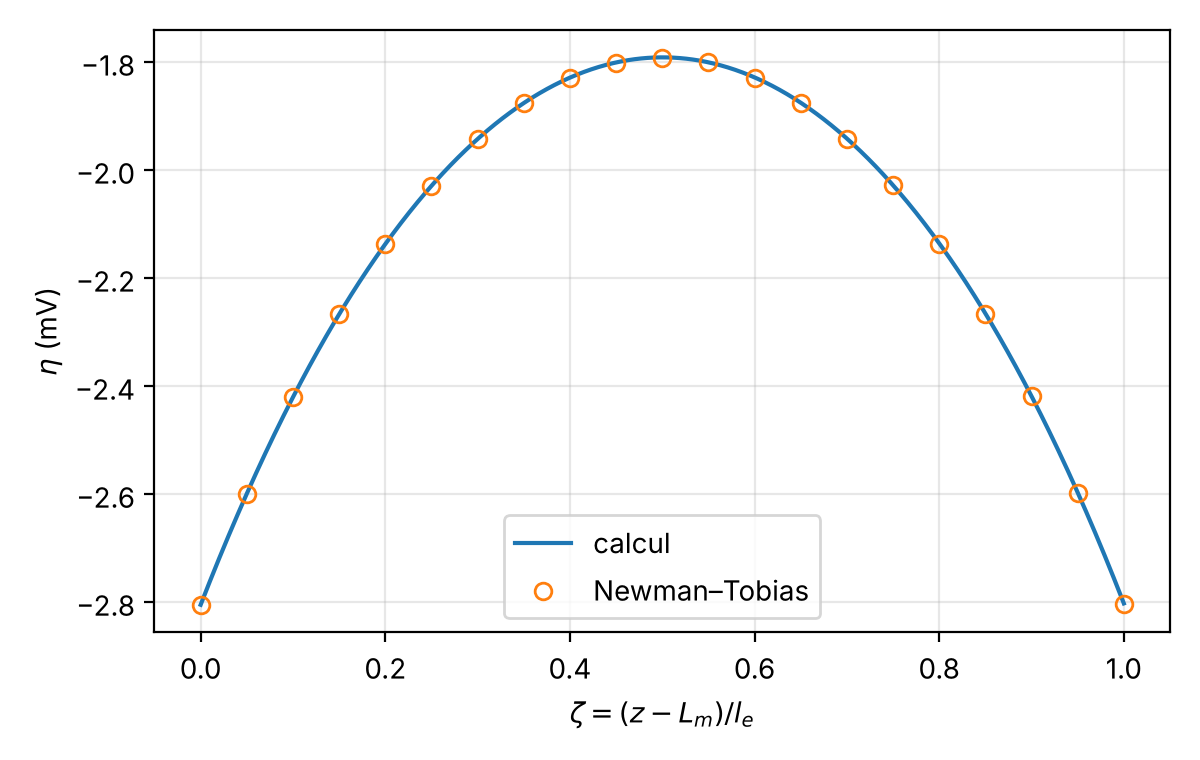
\includegraphics[width=0.6\textwidth]{figures/profils_newman_tobias}
\caption{Cas test de Newman et Tobias : surtension calculée (trait) et
solution analytique~\eqref{eq:ref_NT} (cercles), pour $\Lambda = 2{,}04$,
$K_s/\kappa = 1$ et une tension imposée de $-5$~mV.}
\label{fig:profils_NT}
\end{figure}

\paragraph{Origine de l'écart.} Comme pour Thiele, l'écart ne vient pas de la
discrétisation : il reste le même lorsque le maillage passe de $251$ à
$2001$ nœuds. Il traduit les hypothèses de la solution analytique,
principalement la linéarisation de la loi de Butler--Volmer : il est divisé
par trois lorsque la tension imposée passe de $-5$ à $-1$~mV
(tableau~\ref{tab:ecart_NT}).

\begin{table}[H]
\centering
\begin{tabular}{rrcc}
\hline
$E$ (mV) & $M$ & écart relatif sur $\eta$ & écart relatif sur $I$ \\
\hline
$-5$ & $251$  & $1{,}07\times10^{-4}$ & $1{,}15\times10^{-4}$ \\
$-5$ & $1001$ & $1{,}06\times10^{-4}$ & $1{,}12\times10^{-4}$ \\
$-5$ & $2001$ & $1{,}06\times10^{-4}$ & $1{,}12\times10^{-4}$ \\
$-1$ & $251$  & $3{,}27\times10^{-5}$ & $1{,}82\times10^{-5}$ \\
$-1$ & $1001$ & $3{,}37\times10^{-5}$ & $2{,}18\times10^{-5}$ \\
$-1$ & $2001$ & $3{,}37\times10^{-5}$ & $2{,}20\times10^{-5}$ \\
\hline
\end{tabular}
\caption{Écarts à la solution de Newman et Tobias en fonction de la tension
imposée et du nombre de nœuds.}
\label{tab:ecart_NT}
\end{table}

\paragraph{Ordre de convergence.} Pour faire apparaître l'erreur de
discrétisation, le cas est recalculé avec une tension imposée de
$-0{,}1$~mV, qui rend l'erreur de linéarisation négligeable, et sur des
maillages grossiers. L'écart sur $\eta$ est alors divisé par quatre chaque
fois que le pas est divisé par deux (tableau~\ref{tab:convergence_NT}), ce
qui confirme l'ordre deux du schéma pour la partie conduction. Sur les
maillages plus fins, il se stabilise vers $3\times10^{-5}$, valeur de l'écart
de modèle résiduel.

\begin{table}[H]
\centering
\begin{tabular}{rrcc}
\hline
$h$ (nm) & $M$ & $\max|\eta - \eta^{\mathrm{NT}}|/\max|\eta^{\mathrm{NT}}|$ & ordre \\
\hline
$1000$ & $11$ & $1{,}84\times10^{-3}$ & -- \\
$500$  & $21$ & $4{,}53\times10^{-4}$ & $2{,}02$ \\
$250$  & $41$ & $1{,}04\times10^{-4}$ & $2{,}12$ \\
\hline
\end{tabular}
\caption{Écart à la solution de Newman et Tobias en fonction du pas du
maillage, pour une tension imposée de $-0{,}1$~mV.}
\label{tab:convergence_NT}
\end{table}

\subsubsection*{Bilan de la vérification}

Les deux solutions de référence sont retrouvées, avec des écarts que l'on
sait attribuer aux hypothèses des solutions analytiques et non au code : ils
ne dépendent pas du maillage, et ils diminuent lorsque l'hypothèse
correspondante est mieux satisfaite. Lorsque ces écarts de modèle sont
rendus négligeables, l'écart restant décroît comme $h^2$ dans les deux cas.
Le tableau~\ref{tab:bilan_verif} résume les deux cas tests : chacun isole une
source de perte d'efficacité en rendant l'autre négligeable. Dans les
situations réalistes, où les deux pertes se cumulent et où il n'existe pas de
solution analytique, le calcul s'appuie donc sur deux parties du code
vérifiées séparément.

\begin{table}[H]
\centering
\begin{tabular}{lcc}
\hline
 & Thiele & Newman et Tobias \\
\hline
Grandeur variable & concentrations & surtension \\
Grandeur uniforme & potentiels & concentrations \\
Cinétique & Tafel ($\eta = -0{,}65$~V) & linéaire ($E = -5$~mV) \\
Nombre adimensionnel & $\phi = 1{,}876$ & $\Lambda = 2{,}037$ \\
Efficacité, transport de matière & $\eta_E = 0{,}509$ & $\eta_E \simeq 1$ \\
Efficacité, conduction & $\eta_E^{\mathrm{NT}} \simeq 1$ & $\eta_E^{\mathrm{NT}} = 0{,}42$ \\
Écart maximal & $8\times10^{-4}$ sur $C_{\ce{CO2}}$ & $1{,}1\times10^{-4}$ sur $\eta$ \\
Origine de l'écart & chutes de potentiel & linéarisation \\
Ordre du schéma & 2 & 2 \\
\hline
\end{tabular}
\caption{Synthèse des deux cas tests de vérification.}
\label{tab:bilan_verif}
\end{table}

% ============================================================
\subsection*{Résultats}

La figure~\ref{fig:profils_thiele} présente la solution du cas test. Le
\ce{CO2}, apporté par la phase homogène en $z = L_b$, est consommé à mesure
qu'il pénètre dans l'électrode : sa concentration passe de
$34$~mol\,m$^{-3}$ à l'interface à $10{,}2$~mol\,m$^{-3}$ au collecteur. La
réaction, proportionnelle à la concentration de \ce{CO2}, est donc environ
trois fois plus lente au fond de l'électrode qu'à l'interface, ce que
traduit le facteur d'efficacité $\eta_E = 0{,}51$ : la
moitié environ de la surface catalytique est réellement utilisée. Le \ce{CO}
produit s'accumule au fond de l'électrode, où il atteint
$2{,}8$~mol\,m$^{-3}$, et diffuse vers la phase homogène, où sa concentration
est nulle.

Les potentiels varient très peu, conformément au choix des paramètres :
$\varphi_l$ diminue de $0{,}18$~mV de l'interface au collecteur, sous l'effet
du courant ionique qui traverse l'électrolyte, et $\varphi_s$ augmente de
$0{,}02$~mV du collecteur vers l'interface, sous l'effet du courant
électronique. La surtension est donc pratiquement uniforme, comme le suppose
le modèle de Thiele.

\begin{figure}[H]
\centering
\includegraphics[width=\textwidth]{figures/profils_thiele}
\caption{Solution du cas test. (a) Concentrations de \ce{CO2} et de \ce{CO}
calculées (traits) et solution analytique de Thiele (cercles). (b) Potentiel
électrolytique. (c) Écart du potentiel solide à sa valeur imposée au
collecteur.}
\label{fig:profils_thiele}
\end{figure}